\chapter{基礎知識と課題整理}
\label{chap:background}

\section{sXGPと4G/5Gの概要}
\subsection{sXGPの位置づけ(免許不要・TD-LTE互換)}
\subsection{4G RAN(UE・eNB)とEPC/5GCの要素}
\subsection{5GCのアーキテクチャ(AMF/SMF/UPF等)}

\section{RAN–コア間インターワーキングの基礎}
\subsection{制御面(S1-AP vs. NG-AP)}
\subsection{ユーザ面(GTP-U互換性とパススルー/変換)}
\subsection{ID/コンテキスト管理(NAS, IMSI/SUPI 等)}

\section{モバイルシステム全体での課題感}
\subsection{研究環境のコストとライセンス(免許・機器費用)}
\subsection{相互接続性・ベンダ依存の壁}
\subsection{運用・再現性とオープンテストベッドの不足}
\subsection{セキュリティ・計測基盤の一般化の難しさ}

\section{本研究が対象とする課題の定義}
\subsection{研究者・学生が手軽に再現できる環境の要件}
\subsection{sXGP×5GC接続の技術的論点の範囲}
\subsection{評価指標と成功基準の設定}


% (注)宇宙通信に関する章は本研究スコープ外のため削除。

% (注)該当節を削除。


% (注)該当節を削除。


% (注)該当節を削除。

% (注)DTN記述は別研究のため削除。

% \subsection{通信機会の非対称性}
% \label{subsection:通信機会の非対称性}

% \begin{figure}[tbh]
%     \centering
%     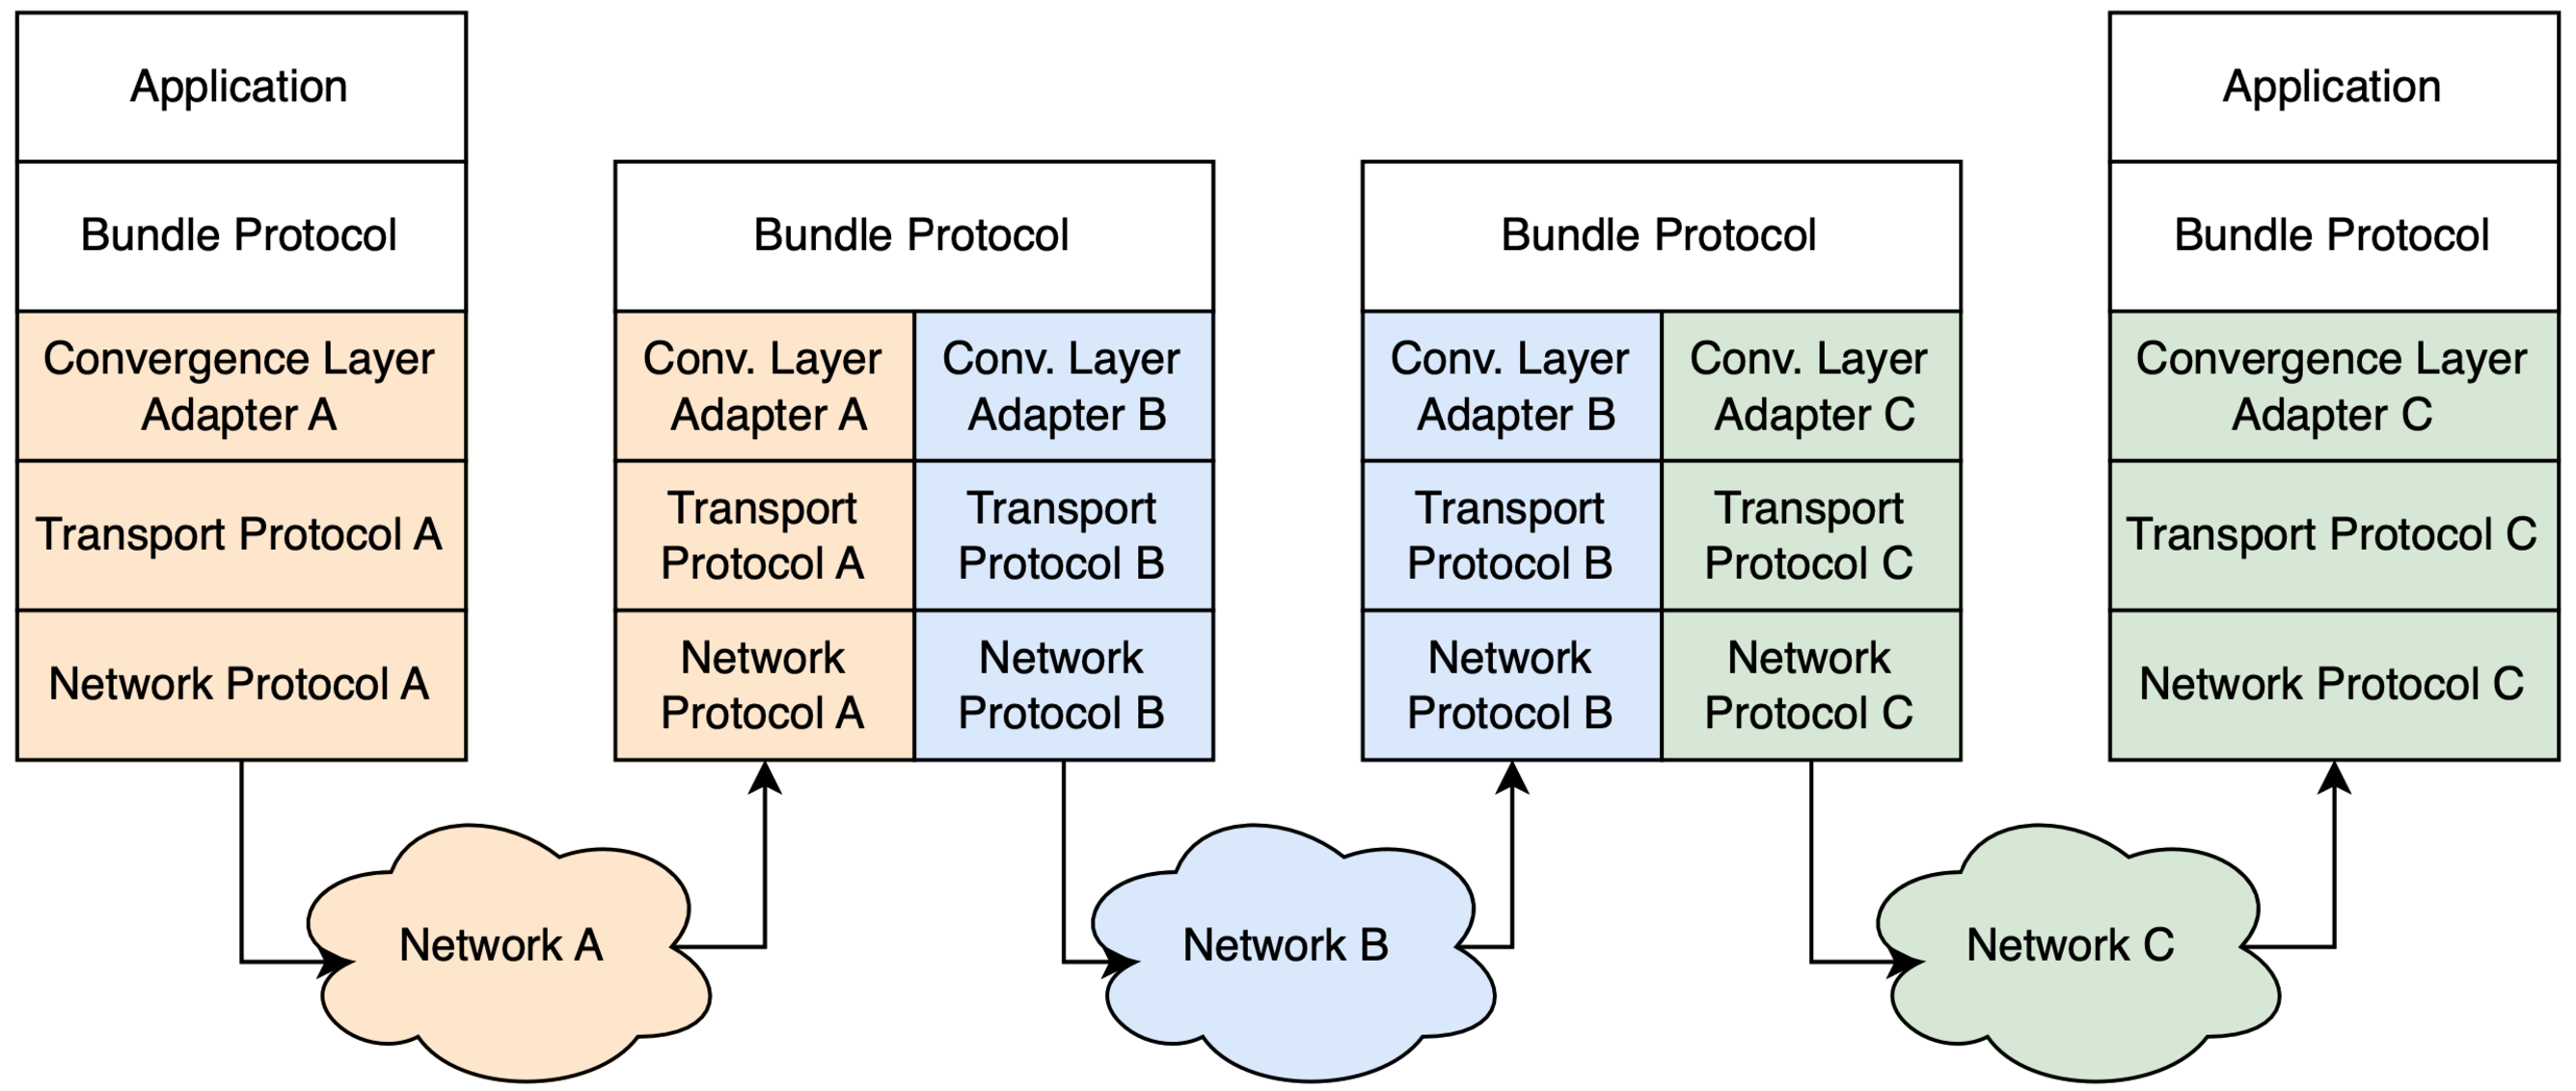
\includegraphics[width=0.7\textheight]{img/dtnprotocolstack.pdf}
%     \caption{DTNを搭載したノード間のみでの通信}
%     \label{fig:dtnprotocolstack}
%     \begin{minipage}{\textwidth}
%         \raggedright
%         \vspace{3mm}
%         \fontsize{10.5pt}{12pt}\selectfont
%         参考文献\cite{bundle_protocol_architecture}Figure1をもとに作成.
%         図中のConvergence Layer(CL)については
%         \ref{section:Convergence LayerとLTP}項で説明する.
%     \end{minipage}
% \end{figure}

% (注)該当節を削除。

% (注)該当節を削除。

% (注)該当節を削除。

% (注)該当節を削除。

% (注)該当節を削除。

% \begin{table}[tbh]
%     \centering
%     \caption{DTN実装とその機能の比較}
%     \begin{minipage}[t]{\textwidth}
%         \centering
%         \fontsize{10.5pt}{12pt}\selectfont
%         参考文献\cite{dtn_implementations}figure1より抜粋
%         \vspace{3mm}
%     \end{minipage}
%     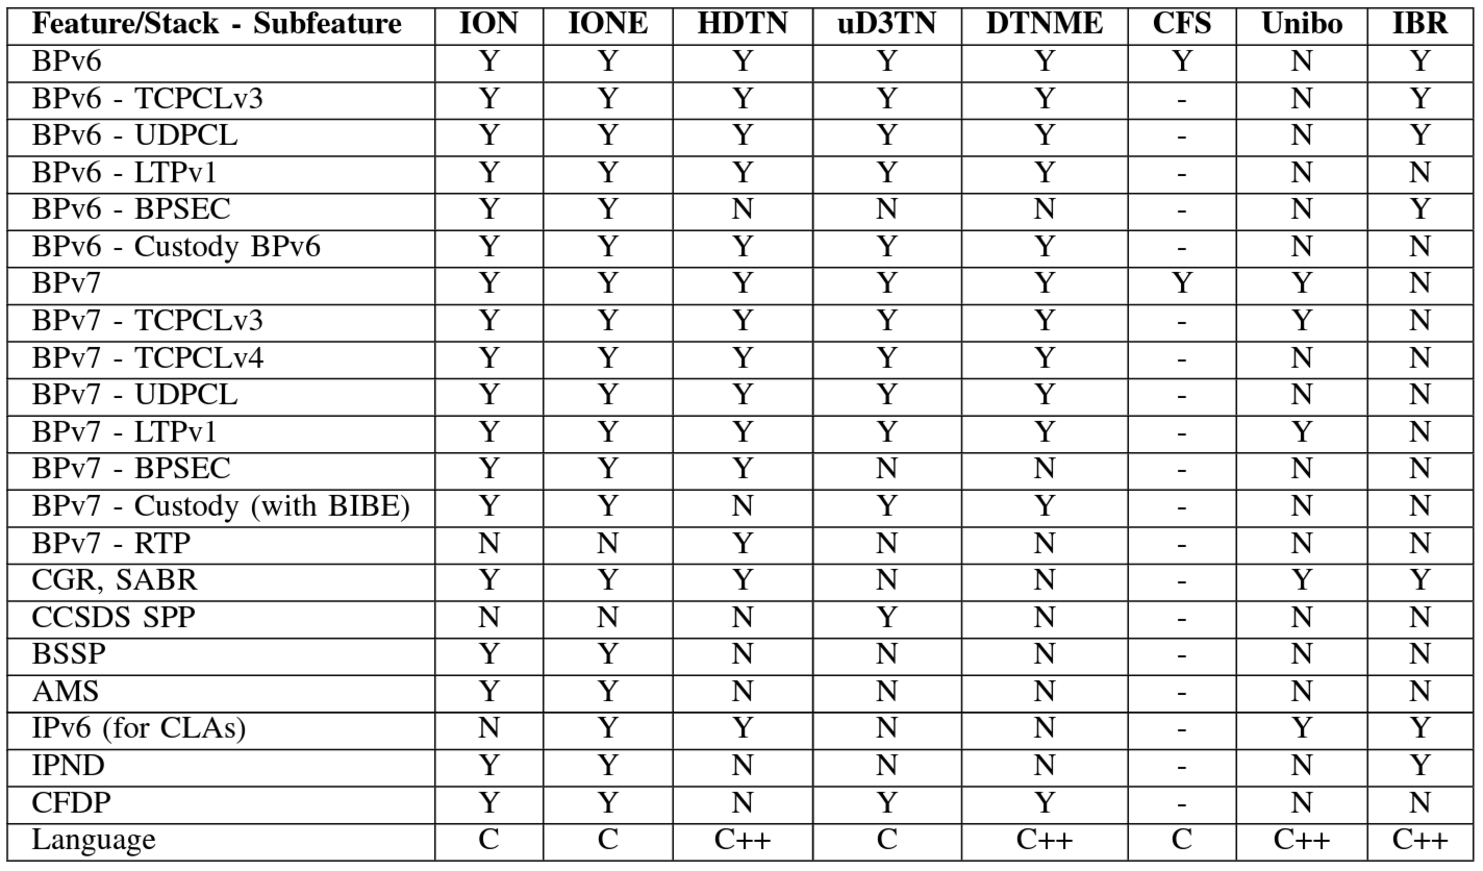
\includegraphics[width=0.7\textheight]{img/chart_dtn_implementations.pdf}
%     \label{table:chart_dtn_implementations}
% \end{table}
